\documentclass[runningheads]{llncs}

\usepackage[T1]{fontenc}
\usepackage[utf8]{inputenc}
\usepackage{amsmath,amssymb}
\usepackage{booktabs}
\usepackage{graphicx}
\usepackage{xcolor}
\usepackage[hidelinks]{hyperref}

% ---- notation, defined once so the symbols cannot drift between sections
\newcommand{\Yo}{Y^{(o)}}          % label frozen at the fresh release, age o
\newcommand{\Yv}{Y^{(v)}}          % label at window close, age v
\newcommand{\pv}{\hat{p}_v}        % teacher's estimate of P(Y^(v)=1 | x)
\newcommand{\wt}{w^{T}}            % teacher's corrector read-out
\newcommand{\NE}{\mathrm{NE}}
\newcommand{\dNE}{\Delta\NE}

\newcommand{\nRuns}{4,850}
\newcommand{\nArms}{37}
\newcommand{\nEval}{8,196,131}
\newcommand{\nCohorts}{719}
\newcommand{\baseRate}{0.1361}
\newcommand{\nLr}{7}
\newcommand{\nContrast}{15}
\newcommand{\capMin}{1,890}
\newcommand{\capMax}{9,580,477}
\newcommand{\teacherParams}{9,456,897}
\newcommand{\seedSdMed}{0.00090}
\newcommand{\seedSdMax}{0.00241}
\newcommand{\nScreened}{11}
\newcommand{\nFail}{8}
\newcommand{\passList}{FSIW, ULC, TWICE}
\newcommand{\maxDup}{4.00}
\newcommand{\maxDupArm}{FTP}
\newcommand{\maxVisits}{97}
\newcommand{\maxVisitsArm}{IF-DFM}
\newcommand{\missDup}{3.05}
\newcommand{\vanillaDup}{1.03}
\newcommand{\collapseSevenBest}{-0.0212}
\newcommand{\collapseSevenWorst}{-0.0055}
\newcommand{\collapseOneBest}{-0.0096}
\newcommand{\collapseOneWorst}{-0.0003}
\newcommand{\collapseSevenSig}{15}
\newcommand{\collapseOneSig}{10}
\newcommand{\collapseSevenMean}{-0.0153}
\newcommand{\collapseOneMean}{-0.0048}
\newcommand{\ratioSeven}{2016}
\newcommand{\ratioOne}{288}
\newcommand{\foSevenFive}{0.265}
\newcommand{\foOneFive}{0.355}
\newcommand{\foOneNinety}{0.803}
\newcommand{\doSmall}{-0.0032}
\newcommand{\doLarge}{+0.0051}
\newcommand{\doSig}{15}
\newcommand{\doSevenLargest}{-0.0028}
\newcommand{\frzOne}{+0.00092}
\newcommand{\frzSeven}{+0.00190}
\newcommand{\frzSevenBeat}{15}
\newcommand{\frzSevenN}{15}
\newcommand{\cdUlcMean}{+0.00050}
\newcommand{\cdUlcNs}{13}
\newcommand{\waitFreshFive}{-0.2066}


\begin{document}

\title{Collapsing the Join Window: Soft Targets for Consolidating\\Fast and Slow Conversions}
\titlerunning{Collapsing the Join Window}

\author{Anonymous}
\institute{Anonymous}
\authorrunning{Anonymous}

\maketitle

\begin{abstract}
Conversion pipelines are segregated by speed: a fast funnel joins on a one-day window, a slow
one on a week or a month, because each must wait for its own label. We ask whether the
\emph{join} delay can be decoupled from the \emph{attribution} window it answers to. A short join records every in-flight conversion as a negative, and most published
corrections repair the record afterwards --- duplicating the event, relabelling it, adding
horizons --- which an append-only log cannot do cheaply: under a single-visit constraint (one
record per click, label frozen when written) \nFail{} of \nScreened{} published methods violate
it, up to \maxDup{} records per click.

What is left is a choice of target. On the public Criteo logs, across five served capacities
(\capMin{}--\capMax{} parameters) and three join delays, replacing a seven-day join with a
five-minute one and letting an offline teacher stand in for the unseen conversions
\emph{improves} $\NE$ in all \nContrast{} cells, by \collapseSevenBest{} to
\collapseSevenWorst{}; at a one-day window the same substitution gains \collapseOneBest{} to
\collapseOneWorst{}. The gain grows as the funnel slows --- the pipelines most worth collapsing
benefit most --- and the teacher may be a shipped artifact rather than a live service. The
collapse is conditional: the record must keep \emph{part} of its hard label. Discarding it
entirely, the most convenient target for a consolidated pipeline, helps only at the smallest
capacities and loses to waiting at the three largest.

\keywords{Conversion rate prediction \and Delayed feedback \and Knowledge distillation
          \and Online learning.}
\end{abstract}

\section{Introduction}
\label{sec:intro}

Conversion pipelines are segregated by speed: a purchase is joined on a one-day window, an
app install or a lead on a week or a month. Each objective gets its own stream because each
must wait for its own label to exist, and is stale by the width of the window it waited for.
Consolidating several objectives into one model therefore meets a pipeline problem before a
modelling one: $K$ objectives with $K$ attribution windows want $K$ records at $K$ times.

The obvious escape is not to wait. Write the record promptly, at a \emph{join delay} $o$ of
minutes rather than days, and accept the label visible then. That label is systematically wrong: every conversion still in flight is recorded as a
negative. A long line of work corrects the
bias~\cite{chapelle2014modeling,yasui2020feedback,yang2021capturing,chen2022asymptotically,ding2026delayed},
but most corrections repair the record after the fact --- duplicating the event when its
outcome arrives, relabelling it, or adding heads at further horizons --- which an append-only
training log cannot do cheaply. We make the restriction explicit as a \emph{single-visit} constraint --- at most one training
record per click, its label frozen when written --- and measure who obeys it: reproducing
\nScreened{} published methods on the Criteo logs, \nFail{} write more than one, up to
\maxDup{} per click (Sect.~\ref{sec:setting}).

What remains is one question: if the record must be written at $o$ and carry one frozen
target, what should that target be? We study four answers --- from the censored outcome,
through the matured one, to targets supplied by an offline teacher --- across five served
capacities and three join delays, and find the segregation unnecessary. Replacing a seven-day join with a five-minute one,
a factor of \ratioSeven{}, and filling the gap with a teacher's estimate \emph{improves} $\NE$
in all \nContrast{} cells we measure, by \collapseSevenBest{} to \collapseSevenWorst{}. At a
one-day window the same substitution gains \collapseOneBest{} to \collapseOneWorst{}. The gain grows as the funnel slows --- the opposite of the usual intuition, and it means the
pipelines most worth collapsing benefit most. The teacher can be a shipped artifact rather than
a live service and still beats the long-join baseline in \frzSevenBeat{} of \frzSevenN{} cells
at seven days.

The collapse is conditional, and the condition is our second finding: the record must keep
\emph{part} of its hard label. Discarding it entirely --- the most convenient target for a
consolidated pipeline, carrying no attribution window at all --- helps only at the smallest
capacities and loses to waiting at the three largest, consistently across join delays.

\section{Setting and the Single-Visit Constraint}
\label{sec:setting}

\subsection{Two delays}

A click $i$ occurs at $C_i$ with features $x_i$ and, if it converts, after a delay $D_i>0$
($D_i=\infty$ otherwise). The \emph{attribution window} $v$ belongs to the objective and fixes
the target $\Yv_i=\mathbf{1}[D_i\le v]$, knowable only at $C_i+v$; the \emph{join delay} $o$
belongs to the pipeline and decides when the record is written, carrying
\begin{equation}
  \Yo_i \;=\; \mathbf{1}\!\left[D_i \le o\right] \;\le\; \Yv_i .
  \label{eq:labels}
\end{equation}
$o=v$ is the segregated status quo; $o\ll v$ is what we want, and the inequality is the price.
We write $F(o)=P(D\le o\mid D\le v)$ for the share of the target's positives visible at write
time. Training runs in hourly rounds --- consume the records released since the last cut-off,
then score every click of the next hour once, retrospectively against $\Yv$ --- so every arm is
judged on the true business label whatever it trained on, and update-then-predict keeps the
evaluation causal.

\subsection{Two rules}

\textbf{Rule 1 (causality).} A record's label must be computable when the record is written and
must not change afterwards. Labelling a record $\Yv$ while writing it at $C_i+o$ uses an outcome
that has not happened --- an upper reference (\textsc{Oracle}), not a system. Strict.

\textbf{Rule 2 (single-visit).} With $n_i$ the number of times click $i$ enters the served
model's loss over its lifetime, Rule~2 requires $\max_i n_i\le 1$. Without it, shortening $o$
is trivial --- write early, write again later --- so Rule~2 is what makes the question
non-empty.

Two choices decide what the screen says: the criterion is $\max_i n_i$, not the mean, since
it is the \emph{existence} of a second write that obliges the pipeline to support one; and the
rule governs the \emph{served} stream, so auxiliaries are not charged. Under a stricter reading
counting any auxiliary fitted on matured labels, the screen would eliminate \textsc{Fsiw},
\textsc{Ulc} \emph{and both of our own arms} alike.

Reproducing \nScreened{} published methods from scratch under one protocol and counting the
records each one's served model consumes per distinct click, \nFail{} write more than
one.\footnote{Two measurement traps, both of which understate duplication. Dividing records
consumed by records released conflates duplication with traffic variation, since a
maturity-gated stream reads clicks from $v$ ago when the click rate differed; the denominator
must be \emph{distinct clicks touched}. And a window shorter than a method's revisit horizon
cannot see the revisit, so we score only clicks whose entire horizon lies inside the stream.
Duplication is a property of emission logic, not of the model: re-running the audit at the
smallest and largest capacities gives identical counts.} Records per click, at $v=1$\,d:
\textsc{DFM}~1.33, \textsc{ES{-}DFM}~1.03, \textsc{DEFUSE}~1.03, \textsc{DDFM}~1.89, \textsc{IF{-}DFM}~2.79, \textsc{FTP}~4.00, \textsc{MISS}~3.05, \textsc{PI}~2.00
\ --- and \maxVisitsArm{} reaches \maxVisits{} writes for a
single click, its mechanism being an update applied whenever a label reverses. The plain
re-ingestion baseline~\cite{ktena2019addressing,gu2021real} measures \vanillaDup{} and fails
the same criterion. Only \passList{} are single-visit: of these \textsc{Fsiw} corrects the
\emph{loss} and \textsc{Twice} adds a head on the conversion clock, both leaving the target
untouched, while \textsc{Ulc} alone changes the target, making it our comparator.

\section{What Fills the Gap}
\label{sec:targets}

Shortening $o$ leaves a gap: conversions arriving between $o$ and $v$ are recorded as
negatives, and something must stand in for them in the record's single frozen target. We study
four answers, identical in pipeline, schedule, features and optimiser, differing only in the
target $\tilde y_i$ and the age $\Delta$ at which the record is written.

\textsc{Fresh} ($\tilde y_i=\Yo_i$ at $\Delta=o$) fills the gap with nothing. \textsc{Wait}
($\tilde y_i=\Yv_i$ at $\Delta=v$) avoids having one by deferring the write: correct label,
$v$-old data. It is the segregated status quo and our
baseline throughout --- a practitioner who refuses both to duplicate records and to train on
wrong labels is already running it. \textsc{Correct-Distill} writes at $\Delta=o$, keeping the realised label and softening only
the observed negatives,
\begin{equation}
  \tilde y_i \;=\; \Yo_i + (1-\Yo_i)\,\wt(x_i),
  \qquad
  \wt(x) \approx P\!\left(\Yv{=}1 \,\middle|\, \Yo{=}0,\, x\right),
  \label{eq:hybrid}
\end{equation}
so an observed positive stays exactly $1$ and only the uncertain mass moves. This is the
functional form of \textsc{Ulc}~\cite{wang2023unbiased}; what differs is the estimator, so a
comparison between them isolates that and nothing else. \textsc{Distill-Only} goes further and regresses on $\pv(x)\approx P(\Yv{=}1\mid x)$ alone:
the record carries features and a number, and no observation at all.

\paragraph{The teacher.} A separate model trained on the \emph{matured} stream --- a record
enters it at $C_i+v$ carrying $\Yv_i$ --- with $\pv$ and $\wt$ as read-outs on one trunk. It is
\emph{evaluated} at the write instant: at $C_i+o$ the student queries it and freezes the number
into the record, so Rule~1 holds even though the target is soft. Softness is not an exemption
from causality, only another way of satisfying it. The construction is distillation from
privileged information~\cite{xu2020privileged}: the teacher sees the matured label, exactly
what the student cannot.

Teacher capacity is fixed at \teacherParams{} parameters for every
student --- training-only, so free at serving time, but it means \emph{served} capacity is
matched across arms while total training capacity is not. And the teacher need not be live:
ours keeps learning from the matured stream, making it a service, whereas frozen after causal
initialisation it is a build-time artifact. We run both. \textsc{Oracle}, writing at $\Delta=o$
but labelling the record $\Yv_i$, violates Rule~1 and bounds what any correction could
recover.

\section{Experimental Setup}
\label{sec:setup}

\paragraph{Data and protocol.} The public Criteo conversion logs released
with~\cite{chapelle2014modeling}. Clicks span 60 days; days $[0,30)$ initialise the model
causally and days $[30,60)$ are the streaming period, divided into \nCohorts{} hourly rounds
giving \nEval{} scored clicks at a base conversion rate of \baseRate{}. Learning rates are
selected per arm and per cell from a \nLr{}-point grid on a held-out slice of the initialisation
period, before any streaming evaluation, and pinned across seeds.

\paragraph{Axes.} Two \emph{attribution windows}, $v=1$\,d and $7$\,d, standing for a fast and a
slow funnel; the contrast between them is the paper's point, so we never average across them and
every comparison is made within one window. Three \emph{join delays}, $o\in\{5,30,90\}$ minutes. Five \emph{served capacities} from
\capMin{} to \capMax{} parameters, scaling embedding tables and interaction trunk together over
more than three orders of magnitude, so a result holding at one size cannot pass as general.
Five seeds everywhere: \nRuns{} runs over \nArms{} arms, of which this paper analyses six.

\paragraph{Metric.} Normalised entropy against $\Yv$, lower better, pooled over all scored
clicks rather than averaged over rounds --- a per-round average normalises each hour by its own
base rate and discards diurnal variation a model can legitimately predict. We report the
difference $\dNE$ between two arms in one cell, since absolute $\NE$ depends on corpus and
capacity.

\paragraph{Statistics.} Seeds differ only in initialisation and minibatch order, so seed $i$
of two arms is a matched pair: paired $t$-test within each cell, Holm--Bonferroni across the
\nContrast{} cells of a contrast. Seed dispersion is small (median $\NE$ sd \seedSdMed{},
maximum \seedSdMax{}), so cells are individually informative. Five seeds measure initialisation
variance on one data origin --- precision, not generalisation.

\section{Results}
\label{sec:results}

Throughout, $\dNE$ is measured against \textsc{Wait} --- the segregated status quo that joins on
the attribution window --- so negative means the short join is better.

\paragraph{The join window can be collapsed.}
Writing the record \ratioSeven{} times sooner than the seven-day window it is accountable to,
and letting the teacher stand in for the conversions not yet seen, lowers $\NE$ in all
\nContrast{} cells --- every one significant --- by \collapseSevenBest{} to
\collapseSevenWorst{} (Fig.~\ref{fig:delta}). At the one-day window the same
substitution gains \collapseOneBest{} to \collapseOneWorst{}, significant in
\collapseOneSig{}.

The two windows differ by a factor of three in the mean (\collapseSevenMean{} against
\collapseOneMean{}), and the direction is the useful part: \emph{the slower the funnel, the
more collapsing its join window is worth}. This inverts the intuition --- a longer window
censors more of the label, so the teacher has more to supply --- because what dominates is the
cost of the alternative: \textsc{Wait} at $v=7$\,d trains on week-old data, and no label
accuracy compensates.

\begin{figure}[t]
\centering
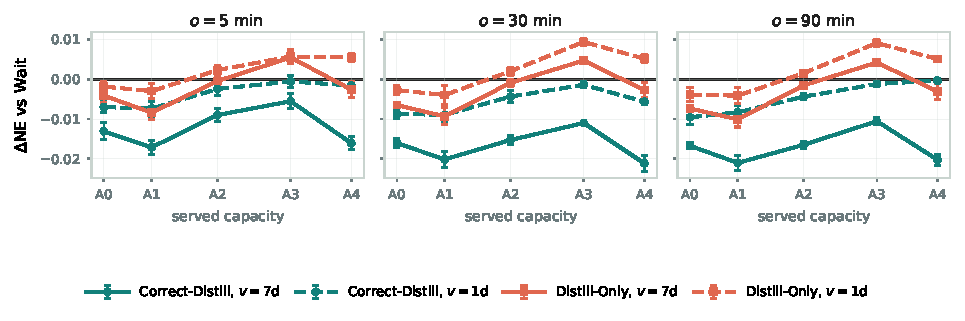
\includegraphics[width=\textwidth]{figs/delta}
\caption{$\dNE$ against \textsc{Wait}; below the line beats the segregated status quo. Colour
is the target, dash the attribution window. \textsc{Correct-Distill} is below the line
everywhere and furthest below at $v=7$\,d; \textsc{Distill-Only} crosses it between A1 and A2
at every join delay when $v=1$\,d. Bars are the standard deviation of the five per-seed
differences.}
\label{fig:delta}
\end{figure}

\paragraph{The condition: keep part of the hard label.}
The collapse above used the hybrid target; the fully soft one decides how far the result can be
pushed. At $v=1$\,d, \textsc{Distill-Only} beats
\textsc{Wait} at the two smallest capacities (\doSmall{} on average) and \emph{loses} at the
three largest (\doLarge{}), crossing over between A1 and A2 at every join delay
(Fig.~\ref{fig:delta}); all \doSig{} cells are significant, so the crossing is not noise. A purely soft target plausibly acts as a regulariser, a variance reduction a small model can
use and a larger one no longer needs~\cite{menon2021statistical}. This cuts against
convenience: a record with no hard label is the most portable object a consolidated pipeline
could ask for, and it is exactly the one that fails at the capacities worth serving. At $v=7$\,d the crossover is weaker and
non-monotone (\textsc{Distill-Only} returns to \doSevenLargest{} at A4), so we state the rule
for the one-day window and do not extrapolate it.

\paragraph{The teacher need not be live.}
Our teacher keeps learning from the matured stream, making it a service rather than an
artifact. Freezing it after causal initialisation costs \frzOne{} $\NE$ at one day and
\frzSeven{} at seven, and frozen \textsc{Correct-Distill} still beats \textsc{Wait} in
\frzSevenBeat{} of \frzSevenN{} cells at seven days: a shipped model, not a running
maturity-gated service, suffices.

\paragraph{Two anchors.}
Two anchors fix the scale. \textsc{Wait} beats \textsc{Fresh} --- the same short join with no
correction --- by \waitFreshFive{} at $o=5$ minutes, so the gap the teacher is filling is an
order of magnitude larger than the gains above, and an uncorrected short join is not an option.
\textsc{Correct-Distill} and \textsc{Ulc}~\cite{wang2023unbiased} share Eq.~\eqref{eq:hybrid}
and differ only in how the corrector is estimated; they are near-indistinguishable (mean $\dNE$ \cdUlcMean{}, \cdUlcNs{} of \nContrast{} cells
not significant at $v=1$\,d). The offline teacher does not beat the online corrector on
accuracy; the case for it is architectural (Sect.~\ref{sec:consolidation}).

\section{What This Means for Consolidation}
\label{sec:consolidation}

Consolidating ranking objectives into one model is an active industrial
direction~\cite{meta2025gem}, and the obstacle is a pipeline one: under \textsc{Wait}
objective $k$'s record exists only at $C_i+v_k$, so a shared append-only stream must either
write $K$ records, violating Rule~2 $K$ times over, or delay everything to $\max_k v_k$ and
impose the slowest funnel's staleness on the fastest. Our result removes the dilemma: one stream at a single short $o$ can
carry $\tilde y_{i,k} = \Yo_{i,k} + (1-\Yo_{i,k})\,\wt_k(x_i)$ for every objective at once,
because $\wt_k$ is a function the pipeline calls rather than an outcome it awaits --- and doing
so is an improvement, most of all for the slow objectives that forced the segregation.

\textsc{Ulc} evaluates at write time too and reaches the same accuracy, so the choice is
architectural. It fits each $w_k$ inside the served model's training loop --- $K$ objectives
become $K$ auxiliaries on one optimiser --- whereas a teacher puts each $w_k$ upstream, its
only interface a number on a record. The frozen result sharpens this: that model can be a
shipped artifact, so consolidation adds $K$ build-time artifacts, not $K$ live services.

\paragraph{What this does not establish.} We ran one objective at a time: no evidence on
interference between objectives sharing a trunk --- the central risk, and what a multi-task
study must measure --- nor that $K$ teachers are affordable at \teacherParams{} parameters
each. Our teacher is comparable in size to our largest student, so small-capacity gains partly
reflect distillation from a larger model; what survives at matched capacity is the smaller
effect. One corpus, one split.

\paragraph{Conclusion.} The join window a pipeline waits for can be decoupled from the
attribution window it is accountable to: shortened by three orders of magnitude, at better
accuracy, with the benefit largest where the funnel is slowest --- provided the record keeps
part of its hard label. The fully label-free target, the most convenient to consolidate, is the
one that fails. The experiment this makes worth running is $K$ heads, $K$ windows, one stream,
teachers upstream.


\bibliographystyle{splncs04}
\bibliography{refs}

\end{document}
